%\chapterauthor{Author Name}{Author Affiliation}
%\chapterauthor{Second Author}{Second Author Affiliation}
\chapter{What is Limit}

\section{The Limit of a Sequence} \label{ch1sec:limitofsequence}

A motivating example of a convergent sequence is given in Section \ref{ch1subsec:sequencemotivatingexample}. The definition of the limit of a sequence is given in Section \ref{ch1subsec:definationoflimitofsequence}. Some useful tricks in proving the convergency of a sequence is given in \ref{chisubsec:proofofsequenceconvergency}. And finally some additional comments are given in \ref{ch1subsec:additionalcommentssequence}.

\subsection{A Motivating Example} \label{ch1subsec:sequencemotivatingexample}

We use $\{a_n\}$ to denote a sequence. In $\{a_n\}$, the positive integer $n$ is the index of the elements in the sequence, where $a_1$ represents the first element of $\{a_n\}$, and $a_2$ the second element, etc.

A sequence has at least one element, and may have in total finite elements (namely, finite sequence) or infinite elements (namely, infinite sequence). In this notebook, we are mostly interested in infinite sequence.

A motivating example is given in Scenario 1 to illustrate the limit of an infinite sequence.

\begin{shortbox}
\Boxhead{Scenario 1}

Consider an infinite sequence $\{a_n\}$ whose elements are recursively derived by
\begin{eqnarray}
  a_1 &=& 1 \label{ch1eq:motivatingexampleinitialcondition} \\
  a_n &=& a_{n-1} + \left(\dfrac{1}{2}\right)^{n-1} \label{ch1eq:motivatingexamplerecursive}
\end{eqnarray}

Q1: Formulate $a_n$ as a function of $n$.

Q2: When will $a_n$ reach/exceed $1.95$? When will $a_n$ reach/exceed $2$? When will $a_n$ reach/exceed reach $3$?
\end{shortbox}

The old school way of solving Q1 in the above scenario is rather simple: use a table to list down different $n$ and its associated $a_n$. The value of $a_n$ can be manually calculated for small $n$, as shown in Table \ref{chi1table:smallan}.

\begin{table}
%\noautomaticrules
\tabletitle{Formulation of $a_n$ as a function of $n$ for small $n$.} \label{chi1table:smallan}
\begin{tabular}{lll}
\tch{$n$}    &\tch{$a_n - a_{n-1}=\left(\frac{1}{2}\right)^{n-1}$} &\tch{$a_n$} \\ \hline
$1$ & --- & $1$ \\
$2$ & $0.5$ & $1.5$ \\
$3$ & $0.25$ & $1.75$ \\
$4$ & $0.125$ & $1.875$ \\
$5$ & $0.0625$ & $1.9375$ \\
$6$ & $0.03125$ & $1.96875$ \\
$7$ & $0.015625$ & $1.984375$ \\
\vdots & \vdots & \vdots
\end{tabular}
\end{table}

With the results presented in Table \ref{chi1table:smallan}, we can also partially answer Q2. Obviously, for any $n\geq6$, variable $a_n$ exceeds $1.95$.

To find out the answers to the rest of Q2, intuitively we probably need a larger table, say Table \ref{chi1table:largean}. Table \ref{chi1table:largean} pushes the digit display limits of most calculators in the market. From Table \ref{chi1table:largean}, it can been seen that as $n$ grows larger and larger, the increment $a_n - a_{n-1} = \left(\frac{1}{2}\right)^{n-1}$ becomes smaller and smaller, and the increment is just not enough to top the next $a_n$ to $2$.

\begin{table}
%\noautomaticrules
\tabletitle{Formulation of $a_n$ as a function of $n$ for larger $n$.} \label{chi1table:largean}
\begin{tabular}{lll}
\tch{$n$}    &\tch{$a_n - a_{n-1}=\left(\frac{1}{2}\right)^{n-1}$} &\tch{$a_n$} \\ \hline
$1$ & $1$ & $1$ \\
$2$ & $0.5$ & $1.5$ \\
$3$ & $0.25$ & $1.75$ \\
$4$ & $0.125$ & $1.875$ \\
$5$ & $0.0625$ & $1.9375$ \\
$6$ & $0.03125$ & $1.96875$ \\
$7$ & $0.015625$ & $1.984375$ \\
$8$ & $0.0078125$ & $1.9921875$ \\
$9$ & $0.00390625$ & $1.99609375$ \\
$10$ & $0.001953125$ & $1.998046875$ \\
$11$ & $0.0009765625$ & $1.9990234375$ \\
$12$ & $0.00048828125$ & $1.99951171875$ \\
$13$ & $0.000244140625$ & $1.999755859375$ \\
$14$ & $0.0001220703125$ & $1.9998779296875$ \\
$15$ & $0.00006103515625$ & $1.99993896484375$ \\
\vdots & \vdots & \vdots
\end{tabular}
\end{table}

An alternative way of finding the solution to Q2 is to derive an analytical equation of $a_n$ as a function of $n$ for any arbitrary $n$. Then we might be able to solve $a_n\geq 2$ and $a_n\geq 3$ for $n$. Notice that
Recursively using \eqref{ch1eq:motivatingexamplerecursive} for $t-1$ times and substituting \eqref{ch1eq:motivatingexampleinitialcondition} into \eqref{ch1eq:motivatingexamplerecursive} gives
\begin{eqnarray}
  a_n &=& \sum_{i=1}^{n} \left(\frac{1}{2}\right)^{i-1} \label{eq:ch1:analyticalv} \\
  &=& 1 + \sum_{i=2}^{n} \left(\frac{1}{2}\right)^{i-1} \label{eq:ch1:analyticalv2}
\end{eqnarray}
and multiplying $\frac{1}{2}$ on \eqref{eq:ch1:analyticalv} gives
\begin{eqnarray}
  \frac{1}{2}a_n &=& \sum_{i=1}^{n} \left(\frac{1}{2}\right)^{i} \nonumber \\
  &=& \sum_{i=2}^{n} \left(\frac{1}{2}\right)^{i-1} + \left(\frac{1}{2}\right)^{n} \label{eq:ch1:analyticalhalfv}
\end{eqnarray}
Subtracting \eqref{eq:ch1:analyticalhalfv} from \eqref{eq:ch1:analyticalv2} gives
\begin{eqnarray}
  \frac{1}{2}a_n &=& 1 - \left(\frac{1}{2}\right)^{n} \nonumber \\
  a_n &=& 2 - \left(\frac{1}{2}\right)^{n-1} \label{eq:ch1:analyticalvresult}
\end{eqnarray}

Equation \eqref{eq:ch1:analyticalvresult} can be verified using the results in Table \ref{chi1table:largean}, and it holds true for any arbitrary $n$. It suggests that the elements in sequence $\{a_n\}$ will not reach 2 let alone 3 for any $n$, as $a_n<2$ for any $n$, although $a_n$ can be very close to $2$ as $n$ increases.

The following features can be observed for sequence $\{a_n\}$:
\begin{itemize}
  \item The sequence is monotonically increasing, as $a_{n-1}<a_n$ for any $n$.
  \item The sequence is bounded, as $a_n<2$ for any $n$.
  \item The sequence can get ``as close to $2$ as we like'', in the sense that for any value smaller than 2, however close to 2 it is (say, 1.9999), $a_n$ will at some point exceeds that value and get even closer to 2, for large enough $n$.
  \item Though both 2 and 3 are upper bounds of $\{a_n\}$ in the context, $2$ is ``special and unique'' to $\{a_n\}$ as $\{a_n\}$ can get ``as close to $2$ as we like''. But this does not apply to $3$ or any value larger than $2$.
\end{itemize}

This existence of sequence $\{a_n\}$ reveals an important yet not intuitive fact that it is possible to find a monotonically increasing yet bounded sequence. Another way to look at it is that it is possible to add infinite number of positive values together, yet the result is bounded.

\subsection{Definition of the Limit of a Sequence} \label{ch1subsec:definationoflimitofsequence}

Given an infinite sequence $\{a_n\}$. If $\{a_n\}$ is bounded and it gets close to a value $L$ ``as close as we like'' for large $n$, then $L$ is called the limit of sequence $\{a_n\}$. To be more precise, the definition of the limit of a sequence is given as follows.

\begin{VF}
\textbf{Definition of the limit of sequence}:
\\
\\
\noindent A sequence $\{a_n\}$ has the limit $L$ if for any $\varepsilon > 0$, there is always a corresponding integer $N$, such that if $n>N$, $|a_n-L|<\varepsilon$. This is denoted by
\begin{eqnarray}
  \lim_{n\rightarrow \infty} a_n &=& L, \nonumber
\end{eqnarray}
or
\begin{eqnarray}
  a_n \rightarrow L  & \textup{as} & n \rightarrow \infty, \nonumber
\end{eqnarray}
and in this case we say ``sequence $\{a_n\}$ is a convergent'' and ``sequence $\{a_n\}$ converges to $L$ as $n$ approaches infinity''.
\end{VF}

The sequence $\{a_n\}$ in \eqref{eq:ch1:analyticalvresult} given in Section \ref{ch1subsec:sequencemotivatingexample} is an example of a convergent sequence that converges to $2$, and we can prove this using the definition of the limit of a sequence as follows. Given any $\varepsilon > 0$, solving
\begin{eqnarray}
  |V(N) - 2| &<& \varepsilon \nonumber
\end{eqnarray}
gives
\begin{eqnarray}
  \left|2-\left(\frac{1}{2}\right)^{N-1}-2\right| &<& \varepsilon \nonumber \\
  N &>& 1-\textup{log}_2\varepsilon \label{eq:ch1:motivatingexamplenrange}
\end{eqnarray}
For example, if specify $\varepsilon = 0.05$, using \eqref{eq:ch1:motivatingexamplenrange} gives $N>5.32$. This implies that from $n\geq 6$ onwards, $|a_n-2|<0.05$ can be obtained. This matches the observation given in Table \ref{chi1table:smallan}.

If an infinite sequence $\{a_n\}$ does not have a limit, we say ``sequence $\{a_n\}$ is divergent'' or ``sequence $\{a_n\}$ diverges''.

As a special case of divergent sequences, if $\{a_n\}$ becomes unbounded as $n$ approaches infinity, we have
\begin{VF}
\textbf{Definition of sequence diverging to infinity}:
\\
\\
\noindent For a sequence $\{a_n\}$, if for any arbitrary positive value $M$, there is always a corresponding integer $N$, such that if $n>N$, $|a_n|>M$, we say ``$\{a_n\}$ diverges to infinity'' and denote it by
\begin{eqnarray}
  \lim_{n\rightarrow \infty}a_n &=& \infty. \nonumber
\end{eqnarray}

\end{VF}

We use $\{s_n\}=\sum_{i=1}^{n}a_n$ to denote the sum of the first $n$ elements in the infinite sequence $\{a_n\}$. Apparently, $\{s_n\}$ itself is also an infinite sequence which may or may not converge depending on $\{a_n\}$. As $n$ approaches infinity, $\{s_n\}$ converges to $\sum_{i=1}^{\infty} a_n$, which is called the infinite sum of the series $\{a_n\}$.

\subsection{Proof of Sequence Convergency} \label{chisubsec:proofofsequenceconvergency}

Proving the convergence/divergence of an infinite sequence and obtaining its limit are sometimes not easy, and need to be done case by case. A few examples are given in the following Table \ref{chi1table:sequencexample} for the convergency of some commonly seen $\{a_n\}$ and its associated sum $\{s_n\}$.

\begin{table}
%\noautomaticrules
\tabletitle{Convergency of commonly seen $\{a_n\}$ and $\{s_n\}$. Variable $c$, $r$ are constant real numbers.} \label{chi1table:sequencexample}
\begin{tabular}{lllcc}
\multirow{2}{*}{\tch{Category}} & \multirow{2}{*}{\tch{$a_n$}} & \multirow{2}{*}{\tch{$s_n$}} & \multicolumn{2}{c}{\tch{Convergency}}  \\
& & & $a_n$ & $s_n$ \\ \hline
Polynomial & $c$ & $nc$ & c & No($\infty$) \\
& $n$ & $\dfrac{n(n+1)}{2}$ & No($\infty$) & No($\infty$) \\
& $n^2$ & $\dfrac{n(n+1)(2n+1)}{6}$ & No($\infty$) & No($\infty$) \\
& $n^3$ & $\dfrac{n^2(n+1)^2}{4}$ & No($\infty$) & No($\infty$) \\
Power Series & $cr^{n-1}, |r|<1$ & $\dfrac{c(1-r^n)}{1-r}$ & $0$ & $\dfrac{c}{1-r}$ \\
Others & $n^{-1}$ & --- & $0$ & No($\infty$) \\
& $n^{-2}$ & --- & $0$ & $\frac{\pi}{6}$ \\
\end{tabular}
\footnotesize{``No($\infty$)'' stands for ``diverges to infinity''.}
\end{table}

If an interested sequence falls in one of the above categories, or at least similar to one of the above categories, or can be expressed as a sum/multiplication/division of two sequences from the above categories, then its convergence/divergence might be proved a bit easier. For example, given two sequences $\{a_n\}$ and $\{b_n\}$, if
\begin{eqnarray}
  \lim_{n\rightarrow\infty} \dfrac{a_n}{b_n} = L \neq 0, \nonumber
\end{eqnarray}
then $\{a_n\}$ and $\{b_n\}$ must behave the same in terms of convergency, meaning that both of them must converge or diverge at the same time.

Some other interesting features regarding sequence convergency are given as follows.

For example, the sum $c_n = a_n + b_n$ of two convergent sequence $\{a_n\}$ and $\{b_n\}$ must be convergent to $\lim_{n \rightarrow \infty}c_n = \lim_{n \rightarrow \infty}a_n + \lim_{n \rightarrow \infty}b_n$. This can be proved using the definition of the limitation of the sequence.

It is intuitive and not difficult to prove that for $\{s_n\}$ to converge, i.e. $\lim_{n\rightarrow\infty}s_n = s$, it is necessary (but not sufficient) for its associated $\{a_n\}$ to converge to zero, i.e. $\lim_{n\rightarrow\infty}a_n = 0$. Do notice that it is possible to have a divergent $\{s_n\}$ even if $\lim_{n\rightarrow\infty}a_n = 0$. An example is the harmonic series given in Table \ref{chi1table:sequencexample} where $a_n = \frac{1}{n}$.

The famous monotone convergence theorem states that \textit{if a sequence $\{a_n\}$ is monotonically increasing or decreasing, and it is at the same time bounded, i.e. $|a_n| < M$ for all $n\geq1$, then $\{a_n\}$ must be convergent}. The proof of this theorem is difficult than it appears to be, thus is not included in the notebook.

From the monotone convergence theorem, we know that for a sequence $\{a_n\}$, if $\sum_{i=1}^{\infty}|a_n|$ converges, then $\sum_{i=1}^{\infty}a_n$ must converge. This is can be illustrated simply by splitting $\{a_n\}$ into $\{a_n^+\}$ and $\{a_n^-\}$, where
\begin{eqnarray}
  a_n^+ &=& \left\{\begin{array}{cc}
                     a_n & a_n \geq = 0 \\
                     0 & a_n < 0
                   \end{array}\right.,  \nonumber \\
  a_n^- &=& \left\{\begin{array}{cc}
                     -a_n & a_n < 0 \\
                     0 & a_n \geq 0
                   \end{array}\right.. \nonumber
\end{eqnarray}

Apparently, $|a_n| = a_n^+ + a_n^-$ and both $\{a_n^+\}$ and $\{a_n^-\}$ are monotonically increasing positive sequences. Since $\sum_{i=1}^{\infty}|a_n|$ is bounded, both $\{a_n^+\}$ and $\{a_n^-\}$ must be bounded, therefore, convergent, according to the monotone convergence theorem. This implies that $a_n = a_n^+ - a_n^-$ must be convergent as the sum of two convergent sequences. If $\sum_{i=1}^{\infty}|a_n|$ converges, then series $\{\sum_{i=1}^{n}a_n\}$ is called ``absolutely convergent''. Absolutely convergent sequence is convergent, but it might be not true wise versa.

\subsection{Additional Comments} \label{ch1subsec:additionalcommentssequence}

There are some famous serious widely used in both mathematics and applied mathematics, such as the famous Taylor serious, which will be introduced in later chapters of the book when the definition of derivative is given. The application of Taylor serious, and many more important serious, can be found in varieties of textbooks related to numerical analysis, signal processing, control engineering, etc., and they will not be covered in details in this notebook.

\section{The Limit of a Function}

\subsection{A Motivating Example} \label{ch1subsec:functionmotivatingexample}

A motivating example is given in Scenario 2 to illustrate the limit of a function.

\begin{shortbox}
\Boxhead{Scenario 2}

Consider function
\begin{eqnarray}
  y = f(x) = \left\{\begin{array}{cc}
                    (x-1)^2 & x \neq 1 \\
                    1 & x = 1
                  \end{array}\right. \label{ch1eq:fxsimple}
\end{eqnarray}

Q1: What is the domain (the set of values for the independent variable $x$) and range (the set of values for the dependent variable $y$) of this function?

Q2: What is the value of $y$ at $x = 1$?

Q3: What is the value of $y$ when $x$ is somewhere close but not equal to $1$ (formally, when $x$ approaches 1)?

\end{shortbox}

We can plot $y$ and $x$ in \eqref{ch1eq:fxsimple}, which shall give as a straight forward impression on what the function looks like. A plot of $y$ as a function of $x$ is given in Fig \ref{ch1fig:fxsimpleexample}. It is clear from the figure that for Q1 the domain and range of the function are $x\in \mathbb{R}$ and $y\in \mathbb{R}, y > 2$ respectively. For Q2, substituting $x=1$ into \eqref{ch1eq:fxsimple} gives $y=1$, as is also illustrated in Fig \ref{ch1fig:fxsimpleexample}.

\begin{figure}
\centering
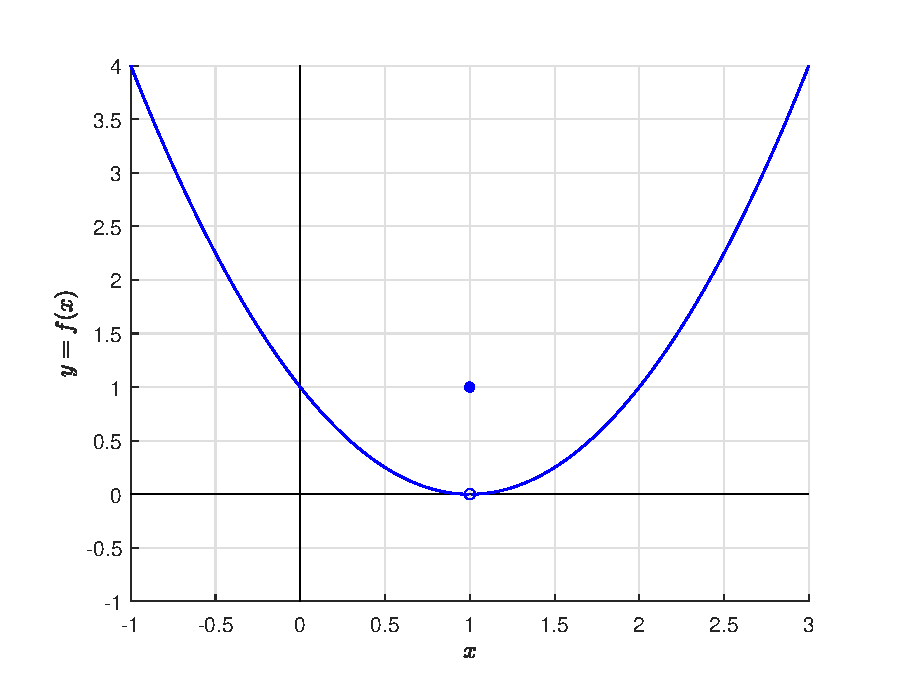
\includegraphics[width=250pt]{chapters/chapter1/figures/fig_fxsimple.eps}
%%\centerline{\epsfig{/Chapters/chapter1/figures/fig_fxsimple.eps,width=.8\textheight,height=.4\textwidth}}
\caption{Plot of $y$ as a function of $x$ in the motivating example.} \label{ch1fig:fxsimpleexample}
\end{figure}

To answer Q3, we need to quantify ``somewhere close but not equal to $1$'' in a more precise manner. An intuitive way of doing that is to define a small ``threshold area'' near $x=1$, say, $-\varepsilon < x-1 < \varepsilon, x \neq 1$. Notice that $x=1$ is out of our concern, which suggests that the value of $y$ near $x=1$ has nothing to do with $y$ at $x=1$. In practice, $\varepsilon$ shall be a rather small positive value as the threshold boundary shall be ``close to $1$''.

Next, we will need to describe $y$ given $-\varepsilon < x-1 < \varepsilon, x \neq 1$. Clearly, the range of $y$ relates to the choice of $\varepsilon$. Substituting $-\varepsilon < x-1 < \varepsilon, x \neq 1$ into \eqref{ch1eq:fxsimple} gives $0 < y < \varepsilon^2$, which is the answer to Q3. If $\varepsilon$ is chosen extremal small, $y$ will approach $0$ (although $y$ cannot be precisely $0$).

\subsection{Definition of the Limit of a Function} \label{ch1subsec:definationoflimitoffunction}

The formal definition of the limit of a function follows the same idea given in Section \ref{ch1subsec:functionmotivatingexample} as follows. Notice that there are a few different but equivalent ways to define the limit of a function. Here the ``epsilon-delta definition'' is introduced.

\begin{VF}
\textbf{Definition of the limit of a function at $x\rightarrow a$}:
\\
\\
\noindent A function $f(x)$ of $x$ has the limit $L$ at $x=a$ if for any $\varepsilon > 0$, there is always a corresponding $\delta > 0$, such that if $|x-a|<\delta$, $|f(x)-L| < \varepsilon$, with prerequisite that $|x-a|<\delta$ is defined for $f(x)$. This is denoted by
\begin{eqnarray}
   \lim_{x\rightarrow a} f(x) &=& L, \nonumber
\end{eqnarray}
or
\begin{eqnarray}
  f(x) \rightarrow L & \textup{as} & x \rightarrow a. \nonumber
\end{eqnarray}
\end{VF}

Using the definition above, it can be proved easily that for Scenario 2 in Section \ref{ch1subsec:functionmotivatingexample} the function has a limit of $\lim_{x\rightarrow 1}f(x)=0$. Do notice that $\lim_{x\rightarrow a}f(x)=L$ does not necessarily require $f(a)=L$. As a matter of fact, $f(x)$ does not need to be defined at $x=a$, as long as it is defined at the neighbour of $x=a$.

Similar to the definition of the limit of a function, the definition of one-sided limit of a function is given below. The two definitions are similar, but the one-sided limit is weaker in the sense that it only requires one side of the neighbour of $x=a$ to be checked.

\begin{VF}
\textbf{Definition of the one-sided limit of a function}:
\\
\\
\noindent A function $f(x)$ of $x$ has the one-side left limit $L_\textup{left}$ at $x=a$ if for any $\varepsilon > 0$, there is always a corresponding $\delta > 0$, such that if $a-\delta<x<a$, $|f(x)-L_\textup{left}| < \varepsilon$, with prerequisite that $a-\delta<x<a$ is defined for $f(x)$. This is denoted by
\begin{eqnarray}
   \lim_{x\rightarrow a^-} f(x) &=& L_\textup{left}, \nonumber
\end{eqnarray}
or
\begin{eqnarray}
  f(x) \rightarrow L_\textup{left} & \textup{as} & x \rightarrow a^-. \nonumber
\end{eqnarray}
\\
\\
\noindent A function $f(x)$ of $x$ has the one-side right limit $L_\textup{right}$ at $x=a$ if for any $\varepsilon > 0$, there is always a corresponding $\delta > 0$, such that if $a<x<a+\delta$, $|f(x)-L_\textup{right}| < \varepsilon$, with prerequisite that $a<x<a+\delta$ is defined for $f(x)$. This is denoted by
\begin{eqnarray}
   \lim_{x\rightarrow a^+} f(x) &=& L_\textup{right}, \nonumber
\end{eqnarray}
or
\begin{eqnarray}
  f(x) \rightarrow L_\textup{right} & \textup{as} & x \rightarrow a^+. \nonumber
\end{eqnarray}
\end{VF}

Clearly from the definition, a function $f(x)$ has a limit of $L$ at $x=a$ if and only if it has both one-sided left limit $L_\textup{left}$ and one-sided right limit $L_\textup{right}$ at $x=a$ and $L_\textup{left}=L_\textup{right}=L$, i.e.
\begin{eqnarray}
  \lim_{x\rightarrow a}f(x)=L &\Leftrightarrow& \lim_{x\rightarrow a^-}f(x) = \lim_{x\rightarrow a^+}f(x) = L. \nonumber
\end{eqnarray}

Furthermore, if function $f(x)$ has a limit $L$ at $x=a$, and also $f(x)=a$, the function $f(x)$ is called continuous function at $x=a$. The example given in Scenario 2 in Section \ref{ch1subsec:functionmotivatingexample} is not continuous at $x=1$ as $\lim_{x\rightarrow 1}=0$ while $\left.f(x)\right|_{x=1}=1$, which can be seen from Fig. \ref{ch1fig:fxsimpleexample}.

The definition of the limit of a function $f(x)$ when $x$ approaches infinity is given below. It is quite similar to the definition of the limit of a infinite sequence.
\begin{VF}
\textbf{Definition of the limit of a function at $x\rightarrow \pm \infty$}:
\\
\\
\noindent A function $f(x)$ of $x$ has the limit $L$ at $x \rightarrow +\infty$ (sometimes denoted as $x \rightarrow \infty$ for simplicity) if for any $\varepsilon > 0$, there is always a corresponding $\delta$, such that if $x > \delta$, $|f(x)-L| < \varepsilon$, with prerequisite that $x > \delta$ is defined for $f(x)$. This is denoted by
\begin{eqnarray}
   \lim_{x\rightarrow +\infty} f(x) &=& L, \nonumber
\end{eqnarray}
or
\begin{eqnarray}
  f(x) \rightarrow L & \textup{as} & x \rightarrow +\infty. \nonumber
\end{eqnarray}
\\
\\
\noindent A function $f(x)$ of $x$ has the limit $L$ at $x \rightarrow -\infty$ if for any $\varepsilon > 0$, there is always a corresponding $\delta0$, such that if $x < \delta$, $|f(x)-L| < \varepsilon$, with prerequisite that $x < \delta$ is defined for $f(x)$. This is denoted by
\begin{eqnarray}
   \lim_{x\rightarrow -\infty} f(x) &=& L, \nonumber
\end{eqnarray}
or
\begin{eqnarray}
  f(x) \rightarrow L & \textup{as} & x \rightarrow -\infty. \nonumber
\end{eqnarray}
\end{VF}

Just like the case of sequence convergency, as a special cases where the function is unbounded, the limit of the function does not exist and we can use $\lim_{x\rightarrow a}f(x) = \pm \infty$ and $\lim_{x\rightarrow \pm \infty}f(x) = \pm \infty$ to represent the cases.

\subsection{Calculation of the Limit of a Function}

The calculation of the limit of many commonly seen elementary functions are often obvious and easy. The limit $\lim_{x\rightarrow a}f(x)$ can very likely be obtained by substituting $x=a$ into the functions, given that the function is defined at $x=a$. The limit $\lim_{x\rightarrow \infty}f(x)$ might be slightly difficult but mostly can be obtained from the definition. Some examples are given below in Table \ref{chi1table:limitoffunction}.

\begin{table}
\tabletitle{Limit of commonly seen elementary functions.} \label{chi1table:limitoffunction}
\begin{tabular}{llll}
\tch{Category} & \tch{$f(x)$} & \tch{$\lim_{x\rightarrow a}f(x)$} & \tch{$\lim_{x\rightarrow \infty}f(x)$} \\ \hline
Polynomial & $p(x)$ & $p(a)$ & No($\infty$) \\
Root & $\sqrt{x}$ & $\sqrt{a}$ for $a>0$ & No($\infty$) \\
Rational & $\dfrac{q(x)}{p(x)}$ & depends & depends \\
Trigonometric & $\textup{sin}(x)$, $\textup{cos}(x)$ & $\textup{sin}(a)$, $\textup{cos}(a)$ & No \\
Exponential & $e^{-x}$ & $e^{-a}$ & $0$ as $x\rightarrow +\infty$, No($\infty$) as $x\rightarrow -\infty$ \\
Logarithm & $\textup{log}_e(x)$ & $\textup{log}_e(a)$ for $a>0$ & No($\infty$) \\
\end{tabular}
\footnotesize{``No($\infty$)'' stands for ``unbounded''; \\
For the case of rational function, if $p(a) \neq 0$, $\lim_{x\rightarrow a}\frac{q(x)}{p(x)} = \frac{q(a)}{p(a)}$. If $p(a)=0$, $\lim_{x\rightarrow a}\frac{q(x)}{p(x)}$ depends on the coefficients of $q(x)$ and $p(x)$ and may not exist. \\
The limit $\lim_{x\rightarrow \infty}\frac{q(x)}{p(x)}$ depends on the order and coefficients of $q(x)$ and $p(x)$ and may not exist.
}
\end{table}

It is worth mentioning a few typical cases where a given function $f(x)$ does not have a limit and/or is not continuous.

Case 1: function $f(x)$ does not converge at a neighbourhood of $x=a$, thus does not have a on-sided limit. For example, consider
\begin{eqnarray}
  f(x) &=& \textup{sin}\left(\dfrac{1}{x}\right). \nonumber
\end{eqnarray}
The function is defined at $x\in\mathbb{R},x\neq0$, but it does not have a one-sided limit $\lim_{x\rightarrow 0^-}f(x)$ or $\lim_{x\rightarrow 0^+}f(x)$, as when $x\rightarrow0$, function $f(x)$ oscillates, as shown in Fig. \ref{ch1fig:sinoneoverx}.

\begin{figure}
\centering
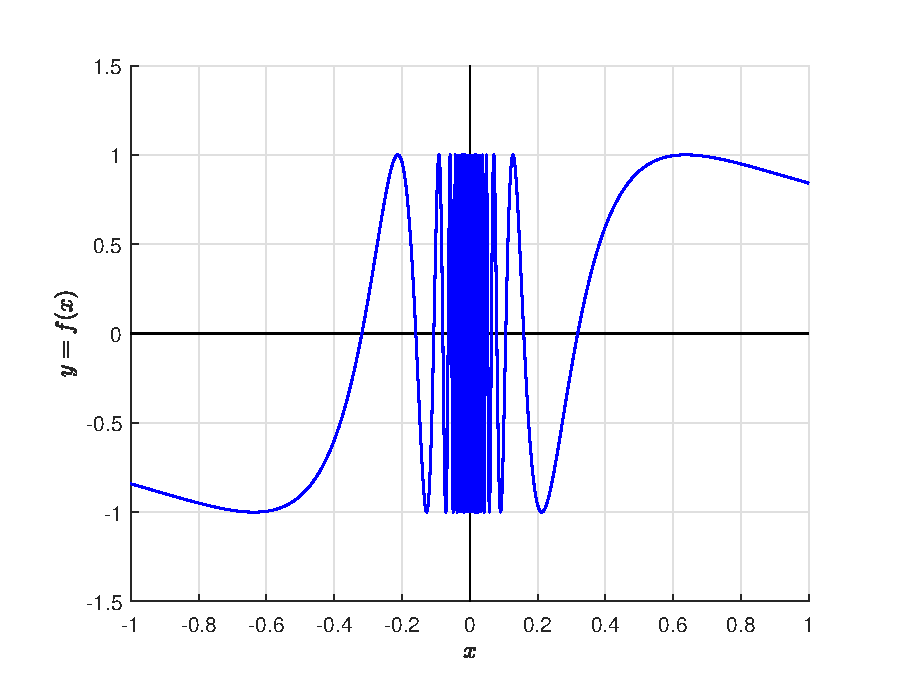
\includegraphics[width=250pt]{chapters/chapter1/figures/fig_sinoneoverx.eps}
%%\centerline{\epsfig{/Chapters/chapter1/figures/fig_fxsimple.eps,width=.8\textheight,height=.4\textwidth}}
\caption{Plot of $y=\textup{sin}\left(\frac{1}{x}\right)$.} \label{ch1fig:sinoneoverx}
\end{figure}

Case 2: function $f(x)$ is unbounded at a neighbourhood of $x=a$, therefore does not have a one-sided limit. For example, consider
\begin{eqnarray}
  f(x) &=& \left|\dfrac{1}{x}\right|. \nonumber
\end{eqnarray}
Apparently, $\lim_{x\rightarrow 0^-}f(x)$ or $\lim_{x\rightarrow 0^+}f(x)$ does not exist.

Case 3: function $f(x)$ has one-sided limit $\lim_{x\rightarrow 0^-}f(x)$ and $\lim_{x\rightarrow 0^+}f(x)$, but $\lim_{x\rightarrow 0^-}f(x) \neq \lim_{x\rightarrow 0^+}f(x)$. For example, consider
\begin{eqnarray}
  f(x) &=& \textup{sign} = \left\{\begin{array}{cc}
                                    1 & x > 0 \\
                                    0 & x = 0 \\
                                    -1 & x < 0
                                  \end{array}\right..\nonumber
\end{eqnarray}
From the definition, $\lim_{x\rightarrow 0^-}f(x)=-1$ and $\lim_{x\rightarrow 0^+}f(x)=1$, therefore, $\lim_{x\rightarrow 0}f(x)$ does not exist.

\subsection{Additional Comments}

The limit of an infinite sequence can be linked to the limit of the associated function at $x\rightarrow\infty$. For example, for sequence $\left\{a_n\right\}$, if $a_n=f(n)$ and $\lim_{n\rightarrow\infty}f(n)=L$, then $\lim_{n\rightarrow\infty}a_n=L$.









